% !TEX TS-program = pdflatex
% !TEX encoding = UTF-8 Unicode

% This is a simple template for a LaTeX document using the "article" class.
% See "book", "report", "letter" for other types of document.

\documentclass[11pt]{article} % use larger type; default would be 10pt

\usepackage[utf8]{inputenc} % set input encoding (not needed with XeLaTeX)

%%% Examples of Article customizations
% These packages are optional, depending whether you want the features they provide.
% See the LaTeX Companion or other references for full information.

%%% PAGE DIMENSIONS
\usepackage{geometry} % to change the page dimensions
\geometry{letterpaper} % or letterpaper (US) or a5paper or....
\geometry{margin=1in} % for example, change the margins to 2 inches all round
% \geometry{landscape} % set up the page for landscape
%   read geometry.pdf for detailed page layout information

\usepackage{graphicx} % support the \includegraphics command and options
\usepackage{hyperref}

\usepackage[parfill]{parskip} % Activate to begin paragraphs with an empty line rather than an indent

%%% PACKAGES
%\usepackage{booktabs} % for much better looking tables
\usepackage{array} % for better arrays (eg matrices) in maths
%\usepackage{paralist} % very flexible & customisable lists (eg. enumerate/itemize, etc.)
\usepackage{verbatim} % adds environment for commenting out blocks of text & for better verbatim
%\usepackage{subfig} % make it possible to include more than one captioned figure/table in a single float
% These packages are all incorporated in the memoir class to one degree or another...

%%% HEADERS & FOOTERS
\usepackage{fancyhdr} % This should be set AFTER setting up the page geometry
\pagestyle{fancy} % options: empty , plain , fancy
\renewcommand{\headrulewidth}{0pt} % customise the layout...
\lhead{}\chead{}\rhead{}
\lfoot{}\cfoot{\thepage}\rfoot{}

%%% END Article customizations

%%% The "real" document content comes below...

\title{Buttons, events, and state machines}
\author{}
\date{} % Activate to display a given date or no date (if empty),
         % otherwise the current date is printed 

\begin{document}
\maketitle

%\begin{quote}
%Wise quote here.\\ \hbox{}\hfil -- {\em A Wise One}
%\end{quote}

\section*{Introduction}

It sounds so easy: the button is either pressed or not. Why all the fuss?

In this lab you’ll explore buttons and switches. You’ll also explore the phenomenon of \emph{bouncing} and learn how to combat it. In the process, you’ll be introduced to event-driven programming, a very useful paradigm for organizing your codes. You’ll finish by making a minimalist home alarm system to prove that you can implement many of the techniques demonstrated in class up to this point.

\subsection*{Objectives}

Upon successful completion of this lab, the student will be able to:
\begin{itemize}
\item Implement an event-driven program for reading a button,
\item Implement button debouncing, 
\item Implement a state machine for reading a keypad, and
\item Demonstrate the application of a number of concepts from the course as a whole.
\end{itemize}

\section*{Preparation}
\subsection*{Background materials}

Review the following materials:
\begin{description}
\item [Switches and debouncing.] In Carryer \emph{et al.}, read Section 13.4 up to and including 13.4.2.
\item [Event-driven programming and state machines.] See readings posted on collab.
\end{description}

\section*{In lab}

\subsection*{Reading a button and debouncing}

Here, you will implement an \emph{event-driven} button counter, explore the bouncing phenomenon, and learn how to combat it. (Note that this was written before we went over some of this in class. You may, for example, already have a decent debouncing code.)

\begin{enumerate}
\item Construct a simple button circuit using the pin of your choice. You may use either an external or internal pull-up resistor.
\item Create a \verb|Button| class that will manage a button interface. The constructor should take the pin that the button is connected to and store it as a data member. What other data members do you need?
\item Write a button checker function to check the button using {\emph event-driven} programming.
\item Separate from the class, write a button handler function that increments a counter whenever the button is pressed and writes the total number of button presses (since the start of the program) to the Serial Monitor. Your \verb|loop()| should look something like:
\begin{verbatim}
void loop()
{
  if(myButton.CheckButtonPress()) HandleButton();
}
\end{verbatim}
where you’ll have to write the (global) \verb|HandleButton()| function.
\item Run your program. Does it work as expected when you press the button 10 times? (Hint: it’s not actually supposed to -- if it does, ask for a demo from an instructor and then carry on with the exercise.)
\end{enumerate}

If the experiment is working -- meaning your code is almost but not quite working right\footnote{You may have already debounced. That’s fine. Attach the oscilloscope and do the following regardless.} -- you should only need to press the button seven or eight times before it says you’ve pressed it ten. This is because the button is \emph{bouncing}. At the microscopic level, every time you push the button or release it, the contacts physically bounce off one another at a very short time-scale, and the processor is fast enough to register the bounces as distinct button presses. You can \emph{debounce} the system with hardware, software, or a combination of the two. You’ll use software after you explore the phenomenon further:

\begin{enumerate}
\item Connect your oscilloscope to the button output and capture a button press. You may need to refresh your memory on how to use triggers. You should see something similar to that in Figure~\ref{fig:bouncing}. Capture 5 - 10 events so that you can see what the longest bouncing duration is -- the worst-case-scenario.
\item Use \verb|delay()| to add a short delay to the code whenever there is a \emph{change} in the button, the length of which should be more than the worst-case-scenario from your oscilloscope captures. Specifically, whenever there is a button transition (either up or down), delay 2 - 3 times as long as the longest button bounce. This will ensure that no bouncing will ever register as a button press, and still be much shorter than the time to actually press a button twice.
\item Run your program and verify that it works.
\end{enumerate}

While \verb|delay| works in this case, it is often not the best solution for many tasks. While the program is executing the \verb|delay()|, it’s unable to do anything else (interrupts excepted -- more on that later). Valuable clock cycles may be wasted doing nothing. A better way is to add a variable to hold the time that the button last changed and only report a button press after a certain amount of time has passed.

\subsubsection*{Skip these two steps for now}

\begin{enumerate}
\item Open the \verb|Debounce| example included with the Arduino IDE. Using the program as a template (only a template -- it’s not a very well written program), write a better debouncing program that doesn’t use \verb|delay()|.
\item Run your program and verify that it works.
\end{enumerate}

{\bf Show your working system to an instructor}, including an oscilloscope capture that shows the bouncing.

\vspace{0.25in}
Instructor initials: \rule{2in}{0.4pt}
\vspace{0.25in}

\begin{figure}
\centering
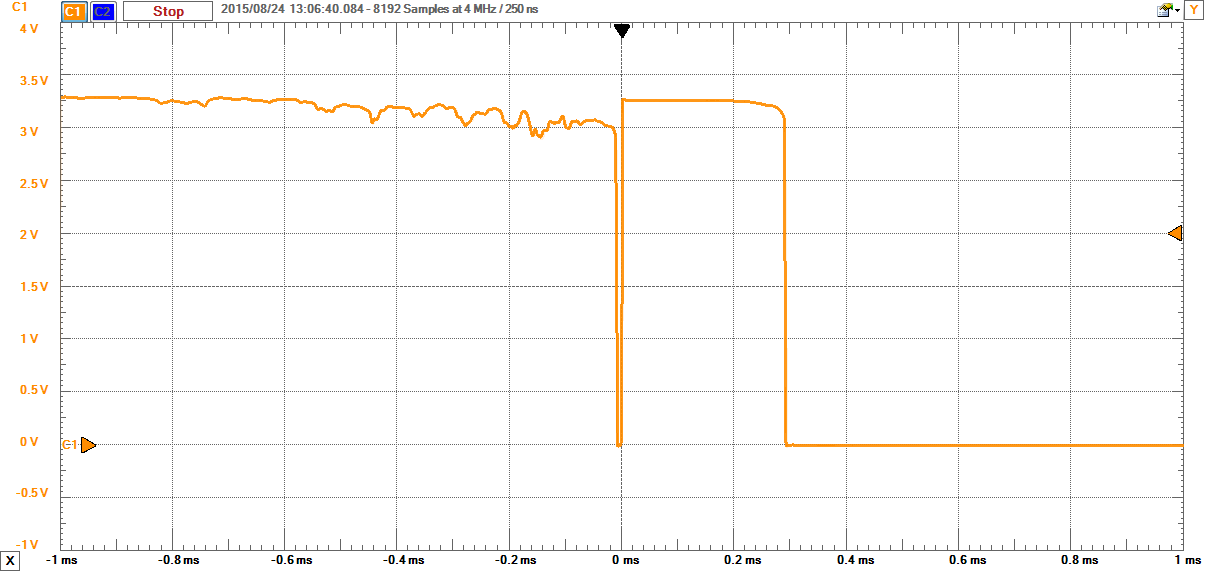
\includegraphics[height=3in ]{figures/bouncing}
%\end{center}
\caption{Pushbutton bounce phenomenon.}
\label{fig:bouncing}
\end{figure}

\clearpage
\section*{Challenge}

Your first challenge project is a minimalist home alarm system. The system will need to allow activation and deactivation; sense an intruder; and sound an alarm if someone is detected. For each of these functions, you’ll use the following hardware and methods:

\begin{description}
\item[ Activation.] To activate your system, one will merely need to press a button. Since you’ll need to have time to close the door after activation, your system will wait 10 seconds after the button is pressed before it activates. You must use a software timer (not \verb|delay()|!) for the timer, since you might want to deactivate it immediately.
\item[ Deactivation.] A simple button will work for activation but it won’t do for deactivation because it would make it easy to defeat the system -- just press the button! Instead, you’ll implement a numeric keypad to deactivate your system. A keypad is just a cleverly arranged set of buttons. Each of the seven pins on the keypad is connected electronically to \emph{either} a column or a row of buttons. Pressing a key will connect two of the pins -- by testing for connections you can see which button has been pressed. Typically, you would change each of the row pins \verb|HIGH| and \verb|LOW| in turn, and check to see if the change is registered on a column pin. {\bf You must be careful not to cause a short circuit, however.} Specifically, you can’t have two row pins as \verb|OUTPUTS| simultaneously.
\item[ Intrusion detection.] When the system is activated, An LED will be lit to represent a laser like you see in the movies. You’ll sense the laser with a photoresistor using the internal comparator (i.e., the last circuit in the previous lab handout). When the beam is occluded, the system will alarm. Note that the laser must be turned off when the system is deactivated.
\item[ Alarming.] Alarming will consist of a blinking LED -- half-second on, half-second off -- and a piezo buzzer that blares at 200 Hz. You must use a software timer for the blinking -- we’ll discuss the buzzer in the coming lectures. You must be able to deactivate the system using the keypad while it’s alarming.
\end{description}

To complete the Challenge, you must do several specific tasks:

\begin{enumerate}
\item Develop a \verb|Keypad| class that manages the interface with the keypad. Among other functions, it should have one called \verb|GetDigit()|, which returns a unique value for each key when pressed.
\item Develop and implement a state machine for decoding a 3-digit (minimum) deactivation code.
\item Develop and implement a state machine for the complete system.
\end{enumerate}

Be sure to follow good coding practices, as we’ve been discussing in class. I promise it will make your lives easier! See an instructor for hints, if you wish.

\subsection*{Deliverables}
For each deliverable, one per team.
\begin{description}
\item[Due 2/12 at the start of class (3 points): ] State diagram for system functionality. Include all states, events, actions, and guard conditions, except you may condense the keypad entry down to “receive valid keycode”. Use proper nomenclature, as from the reading.
\item[Due 2/14 at the start of class (3 points): ] State diagram for keycode entry. The reading gives some examples, but you’ll have to customize them for your system.
\item[Due 2/19 at the start of class (10 points): ] Working system. You’ll have 5 minutes to get your system ready, then I’ll start checking them in random order. I will go through all of the state transitions. Given the time crunch, you will not have time to fix things on the fly -- you get it right or you get it wrong.
\item[Due 2/19 at the start of class (4 points): ] Submit your code, including any custom include files (button.h, keypad.h, rc\_timer.h, etc.), on collab before the start of class. I will grade for style (actual style, like using checker/handler pairs, not faux style like putting your braces in the wrong place or screwing up your capitalization). \verb|delay()| is bad (though allowing in debouncing). Global variables should be used only where needed. Clearly define your state variables. Osv.
\end{description}


\end{document}
